\let\negmedspace\undefined
\let\negthickspace\undefined
\documentclass[journal]{IEEEtran}
\usepackage[a5paper, margin=10mm, onecolumn]{geometry}
\usepackage{tfrupee} 
\setlength{\headheight}{1cm} 
\setlength{\headsep}{0mm}     

\usepackage{gvv-book}
\usepackage{gvv}
\usepackage{cite}
\usepackage{amsmath,amssymb,amsfonts,amsthm}
\usepackage{algorithmic}
\usepackage{graphicx}
\usepackage{textcomp}
\usepackage{xcolor}
\usepackage{txfonts}
\usepackage{listings}
\usepackage{enumitem}
\usepackage{mathtools}
\usepackage{gensymb}
%\usepackage{wasysym}
\usepackage{comment}
\usepackage[breaklinks=true]{hyperref}
\usepackage{tkz-euclide} 
\usepackage{listings}
\def\inputGnumericTable{}                                 
\usepackage[latin1]{inputenc}                                
\usepackage{color}                                            
\usepackage{array}                                            
\usepackage{longtable}                                       
\usepackage{calc}                                             
\usepackage{multirow}                                         
\usepackage{hhline}                                           
\usepackage{ifthen}                                           
\usepackage{lscape}
\usepackage{circuitikz}
\tikzstyle{block} = [rectangle, draw, fill=blue!20, 
    text width=4em, text centered, rounded corners, minimum height=3em]
\tikzstyle{sum} = [draw, fill=blue!10, circle, minimum size=1cm, node distance=1.5cm]
\tikzstyle{input} = [coordinate]
\tikzstyle{output} = [coordinate]
\renewcommand{\thefigure}{\theenumi}
\renewcommand{\thetable}{\theenumi}
\setlength{\intextsep}{10pt} % Space between text and floats
\numberwithin{equation}{enumi}
\numberwithin{figure}{enumi}
\renewcommand{\thetable}{\theenumi}

\begin{document}

\bibliographystyle{IEEEtran}
\vspace{3cm}

\title{5.13.58}
\author{EE25BTECH11032 - Kartik Lahoti}
\maketitle

\subsection*{Question: } 
Let $\omega \neq 1$ be a cube root of unity and $\mathbb{S}$ be the set of all non-singular matrices of the form 

\begin{align}
    \myvec{1 & a & b \\ \omega & 1 & c \\ \omega^2 & \omega & 1}
\end{align}

where each of $a,b$ and $c$ is either $\omega$ or $\omega^2$. Then the number of distinct matrices in the set $\mathbb{S}$ is

\textbf{Solution}:\\


Let,

\begin{align}
    \vec{A} = \myvec{1 & a & b \\ \omega & 1 & c \\ \omega^2 & \omega & 1}
\end{align}

where $\vec{A} \in \mathbb{S}$

For $\vec{A}$ to be Non-singular , $\vec{A}$ should be a full rank matrix.

Thus, 
\begin{align}
    rank\brak{\vec{A}} = 3 
\end{align}


\begin{align}
    \myvec{1 & a & b \\ \omega & 1 & c \\ \omega^2 & \omega & 1} \xleftrightarrow[]{R_2\rightarrow R_2 - \omega R_1 }\myvec{1 & a & b \\ 0 & 1-a\omega & c-b\omega \\ \omega^2 & \omega & 1}
\end{align}

\begin{align}
    \myvec{1 & a & b \\ 0 & 1-a\omega & c-b\omega \\ \omega^2 & \omega & 1} \xleftrightarrow[]{R_2\rightarrow R_2 - \omega^2 R_1 }\myvec{1 & a & b \\ 0 & 1-a\omega & c-b\omega \\ 0 & \omega - a\omega^2 & 1-b\omega^2}
\end{align}

\begin{align}
    \myvec{1 & a & b \\ 0 & 1-a\omega & c-b\omega \\ 0 & \omega - a\omega^2 & 1-b\omega^2} \xleftrightarrow[]{R_3\rightarrow R_3 - \omega R_2 }\myvec{1 & a & b \\ 0 & 1-a\omega & c-b\omega \\ 0 & 0 & 1-c\omega}
\end{align}

For this Row Reduced Echelon Form Matrix to be a full rank matrix, 
the diagonal pivots should be non-zero.

\begin{align}
    1-c\omega \neq 0 \implies c = \omega
\end{align}
\begin{align}
    1-a\omega \neq 0 \implies a = \omega
\end{align}

Non-singularity does not depends on $b$ thus, $b \in \cbrak{\omega , \omega^2} $

\begin{align}
    \therefore n\brak{\mathbb{S}} &= 1 \times 2 \times 1 \\
               n\brak{\mathbb{S}} &= 2
\end{align}

Hence , number of Matrices in Set $\mathbb{S}$ is $2$.

In the graph , Let $1$ be equivalent to $\omega$ and $-1$ be equivalent to $\omega^2$. 

\begin{figure}[H]
    \centering
    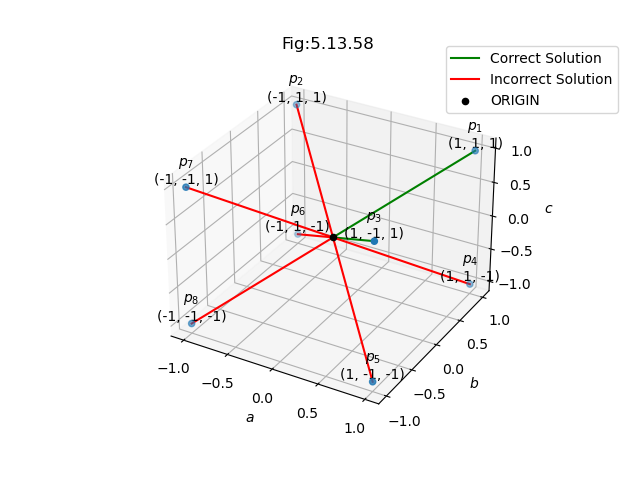
\includegraphics[width=1.0\columnwidth]{figs/vector1.png}
    \caption*{}
    \label{fig:placeholder}
\end{figure}
\end{document}


